\header{
    \headtitle{Le cocu de Paramé} \label{le-cocu-de-parame}
    %
    \insertComment{Chanson enregistrée par Les Frères Jacques datant d'au moins 1959.}{}
}

\enluminure{2}{\href{https://www.youtube.com/watch?v=WYC1MiOxkVA}{S}}{i vous} voulez un' fille,
\\Un' fille à marier,
\\N'allez pas la chercher
\\Au bourg de Paramé,
\\Comme un con !
\\\\\textbf{Refrain :}
\\Ah ! marie-t-on là les filles,
\\Ah ! marie-t-on là les gars!
\\\\N'allez pas la chercher
\\Au bourg de Paramé,
\\Car moi j'en ons pris une
\\Et j'suis ben emmerdé
\\Comme un con !
\\\\Car moi j'en ons pris une
\\Et j'suis ben emmerdé,
\\La premièr' nuit d'mes noces
\\Avec ell' j'ons couché
\\Comme un con !
\\\\La premièr' nuit d'mes noces,
\\Avec ell' j'ons couché,
\\J'y pass' la main su' l'ventre
\\Et j'sentis l'goss' remuer
\\Comme un con !
\\\\J'y pass' la main su' l'ventre,
\\Et j'sentis l'goss' remuer,
\\Je me r'tourn' contr' le mur
\\Et je m'mis à chialer
\\Comme un con !
\breakpage
Je me r'tourn' contr' le mur,
\\Et je m'mis à chialer :
\\« Ne pleur' pas mon p'tit Pierre
\\« Parc' que j't'ons cocufié »
\\Comme un con !
\\\\« Ne pleur' pas, mon p'tit Pierre,
\\« Parce que j 't'ons cocufié,
\\« J't'acat'rons eun' bell' vaque,
\\« Eun' vaqu' ben encornée, »
\\Comme un con !
\\\\« J't'acat'rons eun' bell' vaque,
\\« Eun' vaqu' ben encornée, »
\\« J'y couperions les cornes,
\\« Et j'te les f'rons porter! »
\\Comme un con !
\\\\« J'y couperions les cornes,
\\« Et j'te les f'rons porter,
\\« On dira dans l'village:
\\« V'là l'cocu d'Paramé ! »
\\Comme un con ! 
\bigskip
\begin{center}
   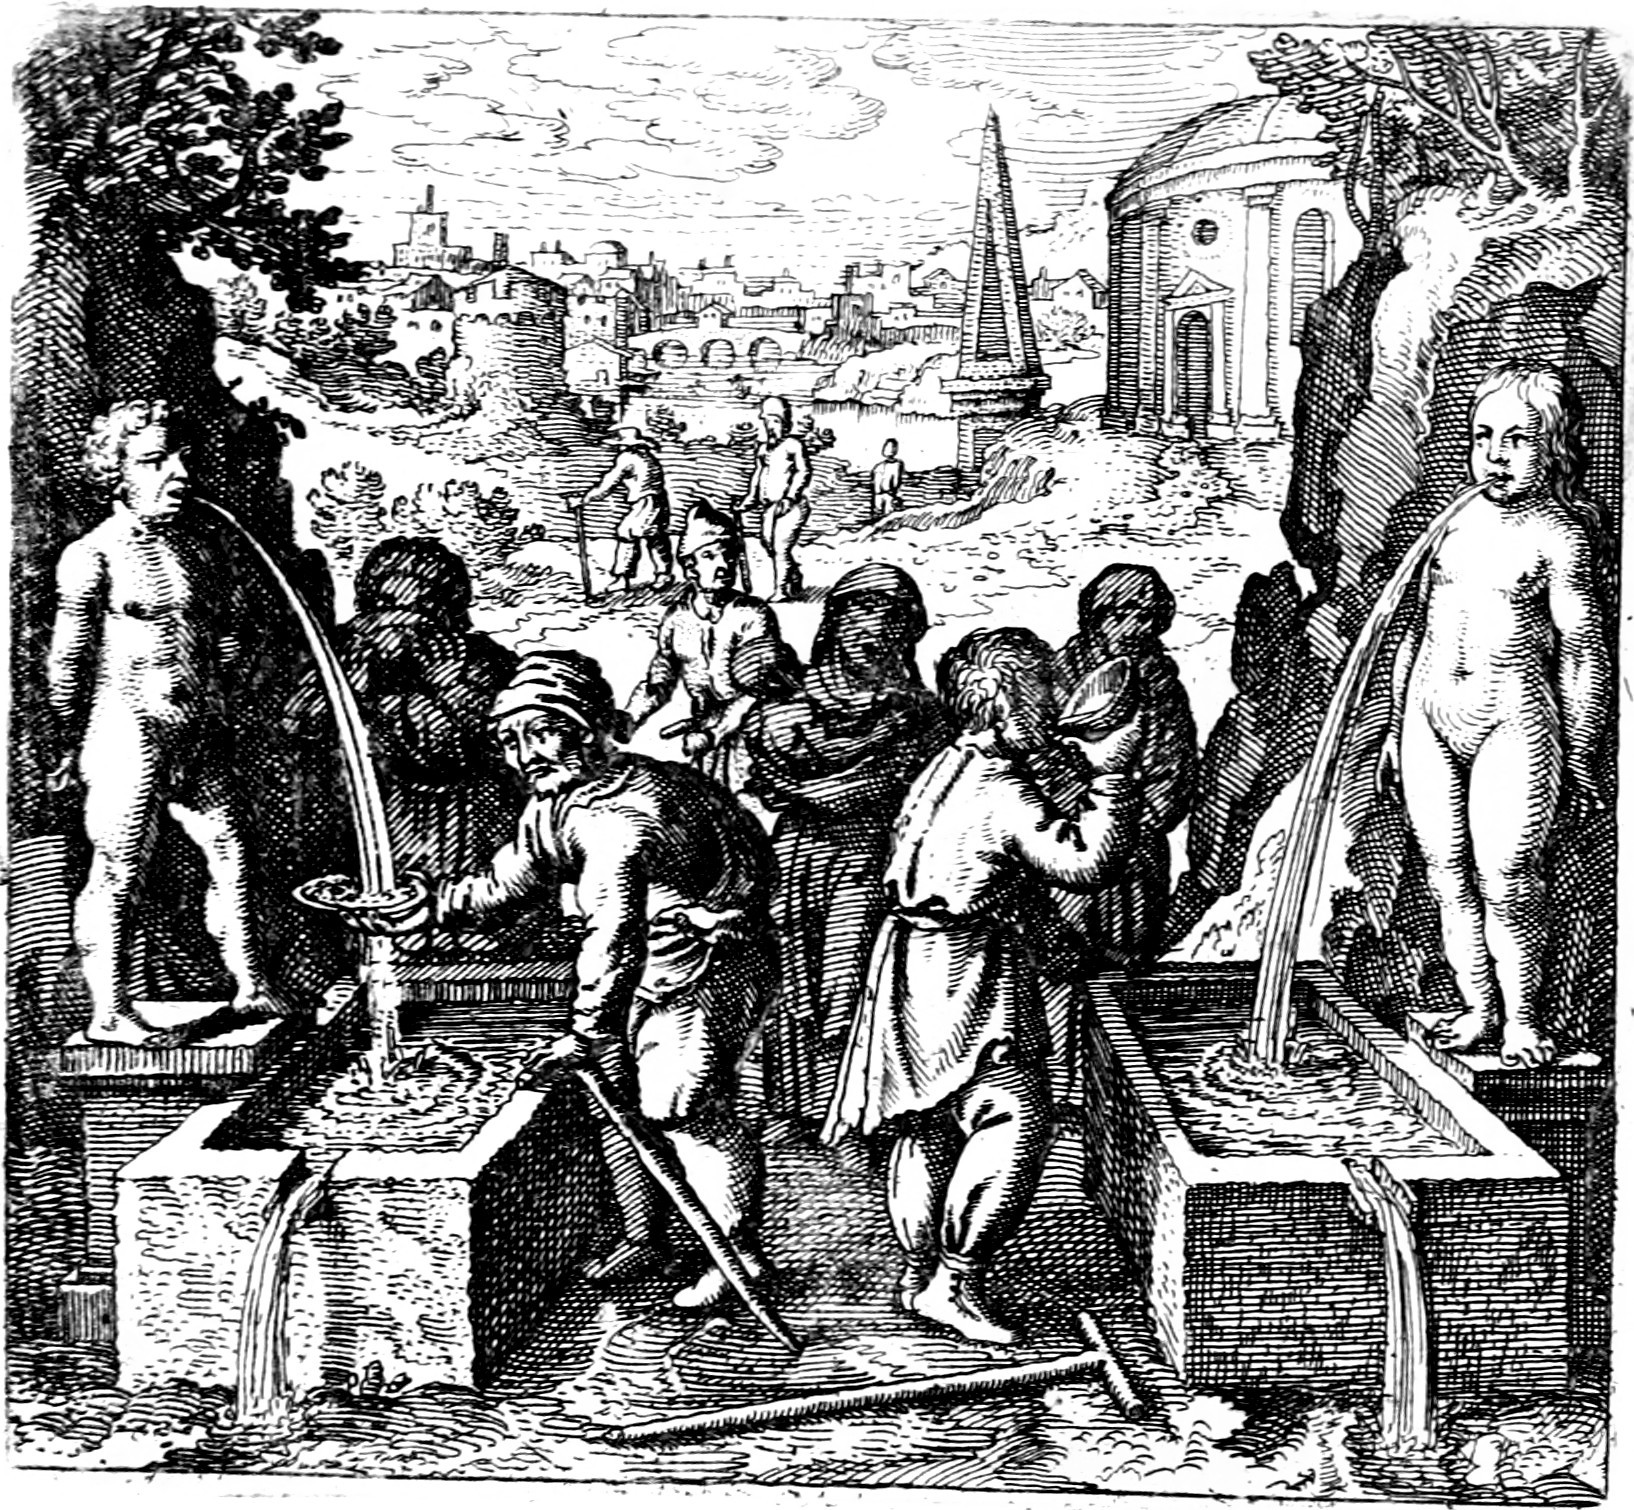
\includegraphics[width=0.7\textwidth]{images/brev42.png}
 \end{center}
 
\breakpage